\documentclass[a4paper,12pt]{extarticle}
\usepackage[utf8x]{inputenc}
\usepackage[T1,T2A]{fontenc}
\usepackage[russian]{babel}
\usepackage{hyperref}
\usepackage{indentfirst}
\usepackage{listings}
\usepackage{color}
\usepackage{xcolor}
\usepackage{here}
\usepackage{array}
\usepackage{multirow}
\usepackage{graphicx}
\usepackage{amsmath}

\hypersetup{
    colorlinks = false,
    linkbordercolor = {white}
}

\definecolor{string}{HTML}{B40000} % цвет строк в коде
\definecolor{comment}{HTML}{008000} % цвет комментариев в коде
\definecolor{keyword}{HTML}{1A00FF} % цвет ключевых слов в коде
\definecolor{morecomment}{HTML}{8000FF} % цвет include и других элементов в коде
\definecolor{сaptiontext}{HTML}{FFFFFF} % цвет текста заголовка в коде
\definecolor{сaptionbk}{HTML}{999999} % цвет фона заголовка в коде
\definecolor{bk}{HTML}{FFFFFF} % цвет фона в коде
\definecolor{frame}{HTML}{999999} % цвет рамки в коде
\definecolor{brackets}{HTML}{B40000} % цвет скобок в коде

\usepackage{caption}
\renewcommand{\lstlistingname}{Программа} % заголовок листингов кода

\bibliographystyle{ugost2008ls}

\usepackage{listings}
\lstset{ %
	extendedchars=\true,
	keepspaces=true,
	language=Python,						% choose the language of the code
	% Цвета
	keywordstyle=\color{keyword}\ttfamily\bfseries,
	%stringstyle=\color{string}\ttfamily,
	stringstyle=\ttfamily\color{red!50!brown},
	commentstyle=\color{comment}\ttfamily\itshape,
	morecomment=[l][\color{morecomment}]{\#},
	basicstyle=\footnotesize,		% the size of the fonts that are used for the code
	numbers=left,					% where to put the line-numbers
	numberstyle=\footnotesize,		% the size of the fonts that are used for the line-numbers
	stepnumber=1,					% the step between two line-numbers. If it is 1 each line will be numbered
	numbersep=5pt,					% how far the line-numbers are from the code
	backgroundcolor=\color{white},	% choose the background color. You must add \usepackage{color}
	showspaces=false				% show spaces adding particular underscores
	keywordstyle=color{blue}\bfseries, 
	showstringspaces=false,			% underline spaces within strings
	showtabs=false,					% show tabs within strings adding particular underscores
	frame=single,          		% adds a frame around the code
	tabsize=2,						% sets default tabsize to 2 spaces
	captionpos=t,					% sets the caption-position to top
	breaklines=true,				% sets automatic line breaking
	breakatwhitespace=false,		% sets if automatic breaks should only happen at whitespace
	escapeinside={\%*}{*)},			% if you want to add a comment within your code
	postbreak=\raisebox{0ex}[0ex][0ex]{\ensuremath{\color{red}\hookrightarrow\space}},
	texcl=true,
	inputpath=listings,                     % директория с листингами
}

\usepackage[left=2cm,right=2cm,
top=2cm,bottom=2cm,bindingoffset=0cm]{geometry}

%% Нумерация картинок по секциям
\usepackage{chngcntr}
\counterwithin{figure}{section}
\counterwithin{table}{section}

%%Точки нумерации заголовков
\usepackage{titlesec}
\titlelabel{\thetitle.\quad}
\usepackage[dotinlabels]{titletoc}

%% Оформления подписи рисунка
\addto\captionsrussian{\renewcommand{\figurename}{Рисунок}}
\captionsetup[figure]{labelsep = period}

%% Подпись таблицы
\DeclareCaptionFormat{hfillstart}{\hfill#1#2#3\par}
\captionsetup[table]{format=hfillstart,labelsep=newline,justification=centering,skip=-10pt,textfont=bf}

%% Путь к каталогу с рисунками
\graphicspath{{fig/}}

\begin{document}	% начало документа

% Титульная страница
%\begin{titlepage}	% начало титульной страницы

	\begin{center}		% выравнивание по центру

		Санкт-Петербургский Национально Исследовательский Университет\\
		информационных технологий, механики и оптики \\
		Кафедра систем управления и информатики\\[3cm]
		% название института, затем отступ 6см
		
		\huge \textbf{РЕФЕРАТ}\\[0.5cm]
		\large Электромеханические системы\\[0.1cm]
		\large Система автоматического управления квадракоптера Parrot ARDrone 2.0\\[2cm]

	\end{center}


	\begin{flushright} % выравнивание по правому краю
%		\begin{minipage}{0.5\textwidth} % врезка в половину ширины текста
%			\begin{flushleft} % выровнять её содержимое по левому краю

				\large Выполнили студенты группы P3335\\
				\large А.М. Зенкин\\[0.5cm]
				\large К.В. Карпов\\[0.5cm]
				
				\large Принял  к.т.н., доцент кафедры СУиР\\
				\sign[4cm]\large  М.С. Чежин\\
				\large Оценка: \sign\\
				«\underline{\hspace{0.7cm}}» \underline{\hspace{2cm}} \the\year г.

%			\end{flushleft}
%		\end{minipage}
	\end{flushright}
	
	\vfill % заполнить всё доступное ниже пространство

	\begin{center}
	\large Санкт-Петербург\\
	\large \the\year % вывести дату
	\end{center} % закончить выравнивание по центру

\thispagestyle{empty} % не нумеровать страницу
%\end{titlepage} % конец титульной страницы
\newpage


% Содержание
% Содержание
\renewcommand\contentsname{\centerline{Содержание}}
\tableofcontents
\thispagestyle{fancy}
\newpage




\section{Цель работы}
Изучение команд для скачивания файлов из Интернета. Изучение команд для работы с архивами. Изучение команд для поиска файлов и слов в файлах.

\section{Задание 1 Скачивание файлов из интернета с использованием терминала:}

\subsection{wget - команда позволяет загружать файлы из сети Интернет. Поддерживает протоколы HTTP, FTP и HTTPS, а также поддерживает работу через HTTP прокси-сервер.}

\begin{figure}[H]
	\begin{center}
		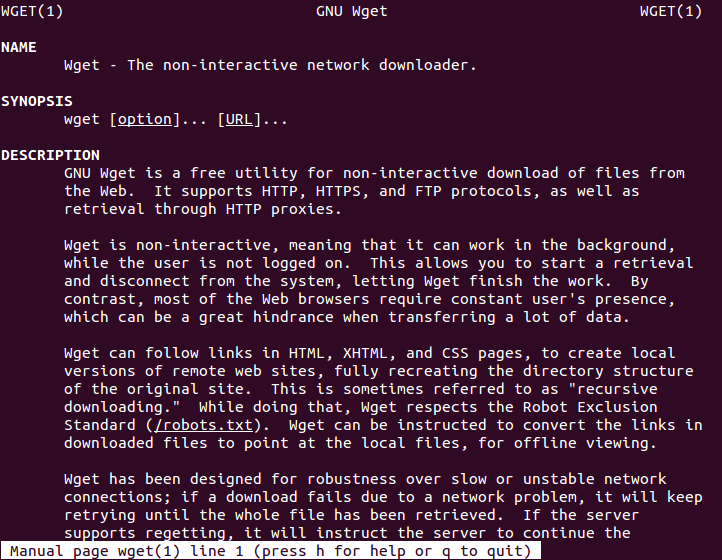
\includegraphics[scale=0.5]{1_1}
		\caption{Отображаем справку команды wget} 
		\label{pic:pic_1} % название для ссылок внутри кода
	\end{center}
\end{figure}

\subsubsection{Параметр --spider проверяет ссылки на доступность}
\subsubsection{Параметр -i даёт возможность работать со ссылками из файлов}

\begin{figure}[H]
	\begin{center}
		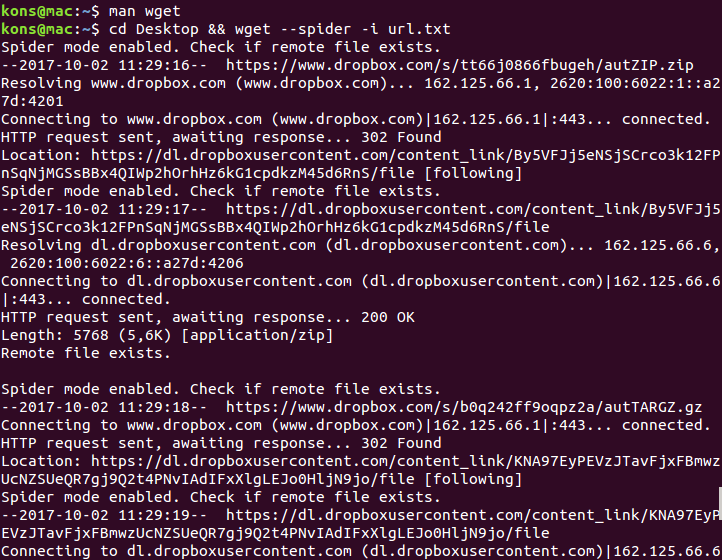
\includegraphics[scale=0.5]{1_2}
		\caption{Проверяем доступность ссылок находящихся в файле} 
		\label{pic:pic_1} % название для ссылок внутри кода
	\end{center}
\end{figure}

\subsubsection{Описание - после команды wget следует ссылка на файл.}

\begin{figure}[H]
	\begin{center}
		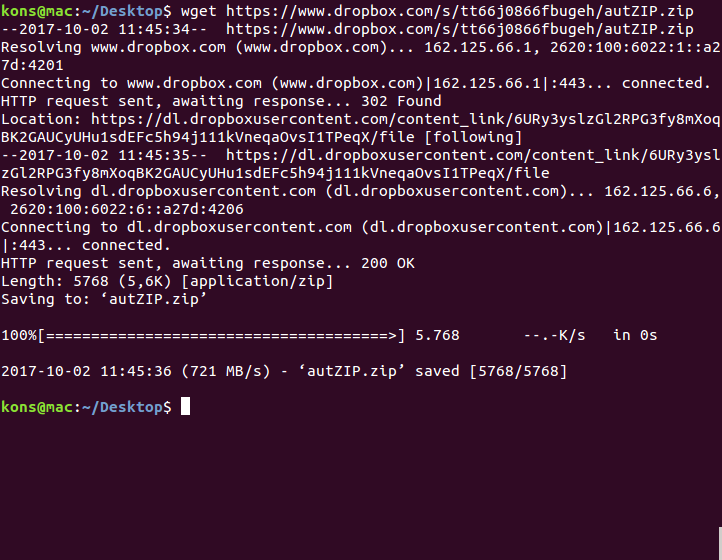
\includegraphics[scale=0.5]{1_3}
		\caption{Скачиваем первый в списке доступный файл} 
		\label{pic:pic_1} % название для ссылок внутри кода
	\end{center}
\end{figure}

\begin{figure}[H]
	\begin{center}
		
\includegraphics[scale=0.5]{1_4}
		\caption{Создаём в домашней папке директорию lab2} 
		\label{pic:pic_1} % название для ссылок внутри кода
	\end{center}
\end{figure}
 
\subsubsection{Параметр -P позволяет сохранять файлы в каталог}
\subsubsection{Параметр -O позволяет менять имя скаченного файла}

\begin{figure}[H]
	\begin{center}
		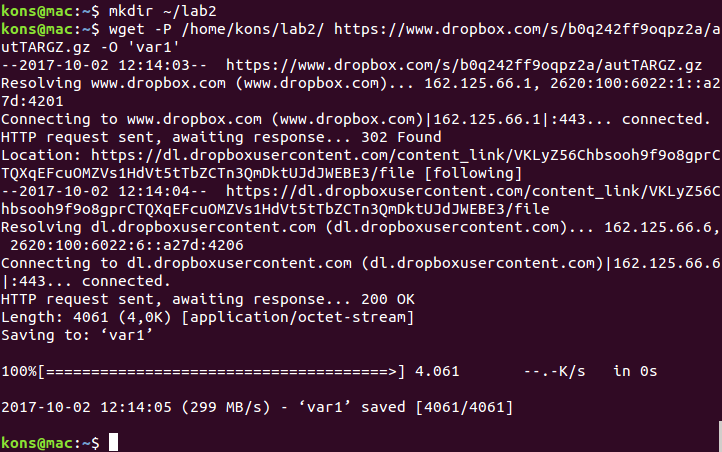
\includegraphics[scale=0.5]{1_5}
		\caption{Скачиваем второй файл в lab2, изменяем имя на 'var1'} 
		\label{pic:pic_1} % название для ссылок внутри кода
	\end{center}
\end{figure} 
 
\begin{figure}[H]
	\begin{center}
		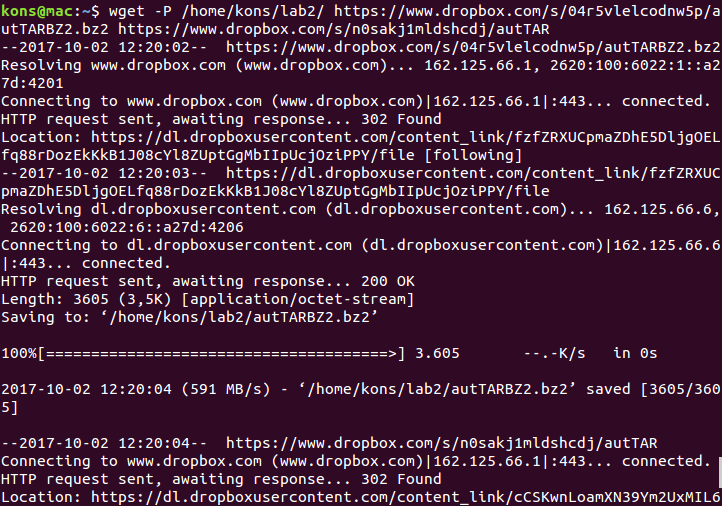
\includegraphics[scale=0.5]{1_6}
		\caption{Скачиваем остальные файлы в директорию lab2} 
		\label{pic:pic_1} % название для ссылок внутри кода
	\end{center}
\end{figure}

\subsubsection{Параметр -r позволяет рекурсивно загружать файлы с сайта}
\subsubsection{Параметр --level=1 устанавливает глубину рекурсии равную единице. Это значит, будут скачиваться файлы находящиеся на данной странице, без перехода в глубь}
\subsubsection{Параметры -A jpeg jpg позволяют скачать файлы с соответствующими форматами}
\subsubsection{Парметр -nd запрещает создавать директории}

\begin{figure}[H]
	\begin{center}
		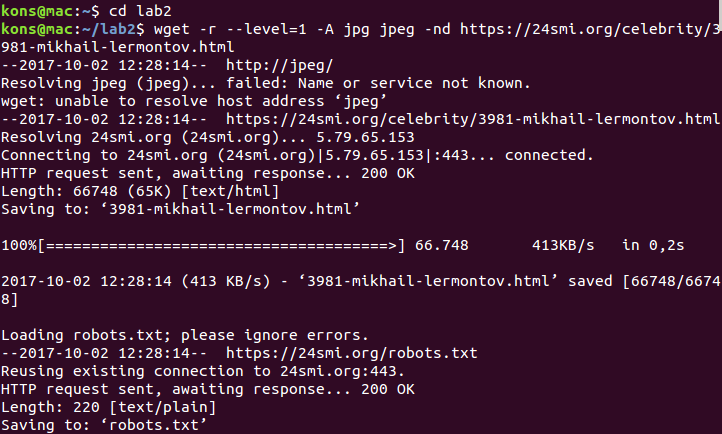
\includegraphics[scale=0.5]{1_7_1}
		\caption{Скачиваем все .jpeg и .jpg файлы с сайта. Часть 1} 
		\label{pic:pic_1} % название для ссылок внутри кода
	\end{center}
\end{figure}

\begin{figure}[H]
	\begin{center}
		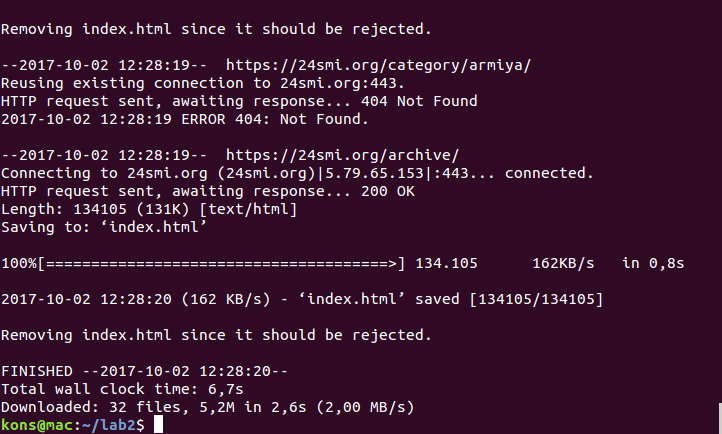
\includegraphics[scale=0.5]{1_7_2}
		\caption{Скачиваем все .jpeg и .jpg файлы с сайта. Часть 2} 
		\label{pic:pic_1} % название для ссылок внутри кода
	\end{center}
\end{figure}

\newpage

\section{Задание 2. Работа с архивами:}

\subsection{unzip - утилита позволяет извелкать файлы из архивов}

\begin{figure}[H]
	\begin{center}
		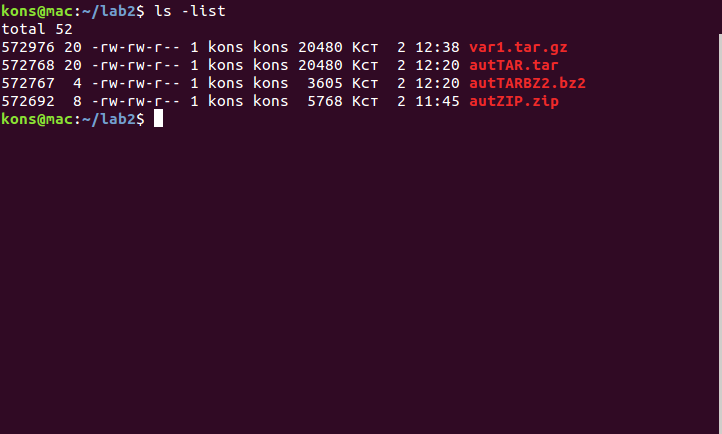
\includegraphics[scale=0.5]{2_2}
		\caption{С помощью команды ls проверяем форматы архивов} 
		\label{pic:pic_1} % название для ссылок внутри кода
	\end{center}
\end{figure}

\subsubsection{Параметр -p позволяет извлечь файлы без сообщений}

\begin{figure}[H]
	\begin{center}
		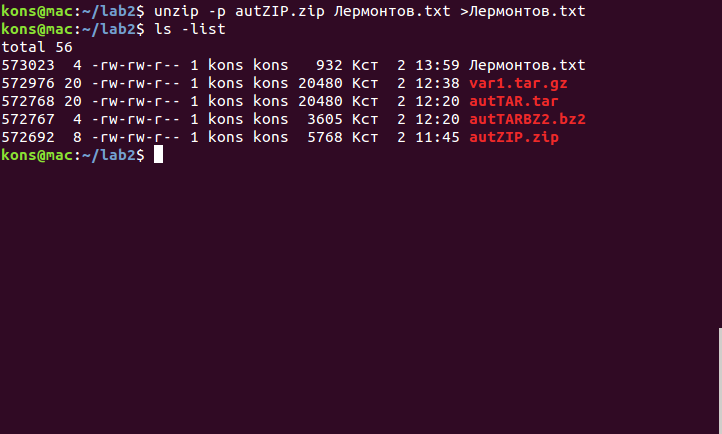
\includegraphics[scale=0.5]{2_3}
		\caption{Извлекаем архив} 
		\label{pic:pic_1} % название для ссылок внутри кода
	\end{center}
\end{figure}

\subsubsection{Параметры -xf позволяют извлечь содержимое архива}
\subsubsection{Параметр -v повзоляет выводить информацию о выполняемых действиях}

\begin{figure}[H]
	\begin{center}
		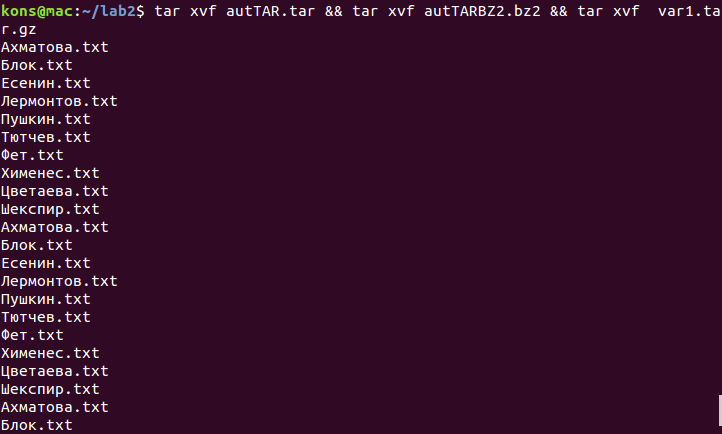
\includegraphics[scale=0.5]{2_4_1}
		\caption{C помощью утилиты tar извлечем все файлы из архивов} 
		\label{pic:pic_1} % название для ссылок внутри кода
	\end{center}
\end{figure}

\newpage

\section{Задание 3. Поиск файлов, поиск по тексту:}

\subsection{find - утилита поиска файлов по имени и другим свойствам, используемая в Unix-подобных операционных системах}

\subsubsection{Параметр -maxdeth указывает глубину проверки}
\subsubsection{Параметр -mtime ищет файлы, с которыми производились действия меньше дня назад}

\begin{figure}[H]
	\begin{center}
		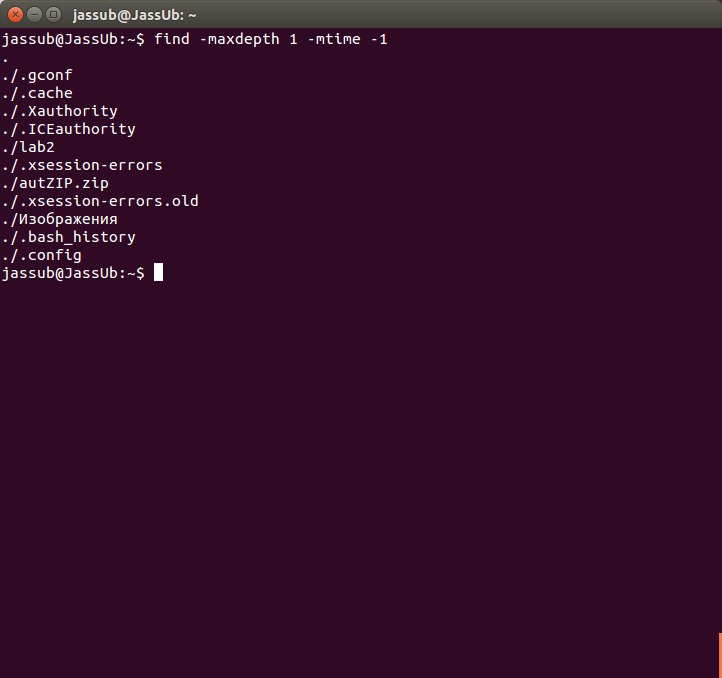
\includegraphics[scale=0.5]{3_1}
		\caption{Найти все файлы, созданные в домашней папке за последний день} 
		\label{pic:pic_1} % название для ссылок внутри кода
	\end{center}
\end{figure}

\subsubsection{Параметр -name позволяет искать файлы по имени}

\begin{figure}[H]
	\begin{center}
		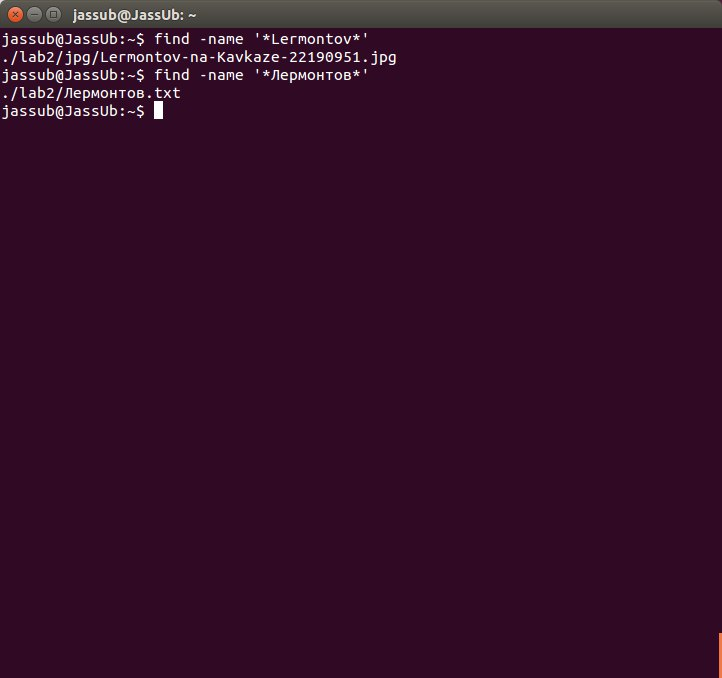
\includegraphics[scale=0.5]{3_2}
		\caption{Найти все файлы c фамилией автора} 
		\label{pic:pic_1} % название для ссылок внутри кода
	\end{center}
\end{figure}

\subsubsection{Параметр -exec используется для указания действий, которые будут выполнены при нахождении файла с именем, удовлетворяющим выражению поиска}

\begin{figure}[H]
	\begin{center}
		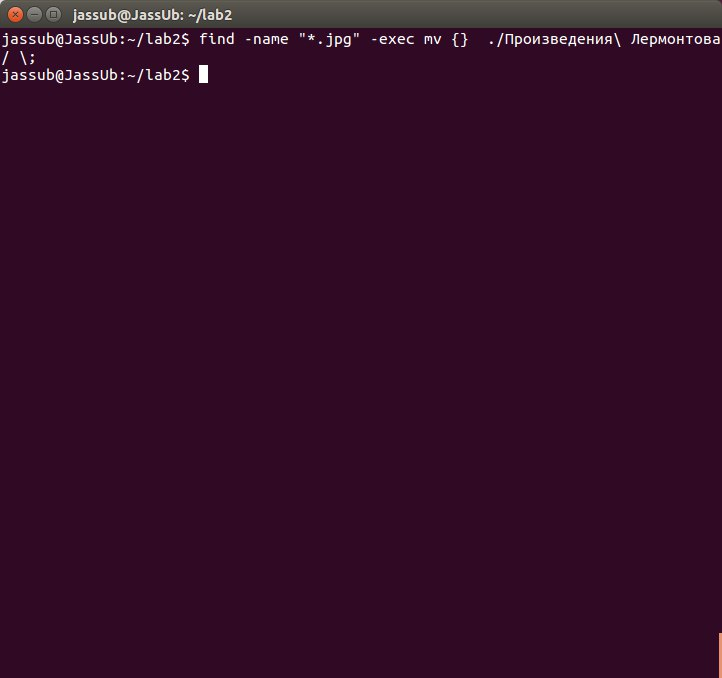
\includegraphics[scale=0.5]{3_3}
		\caption{Находим и перемещаем все *.jpg файлы} 
		\label{pic:pic_1} % название для ссылок внутри кода
	\end{center}
\end{figure}

\begin{figure}[H]
	\begin{center}
		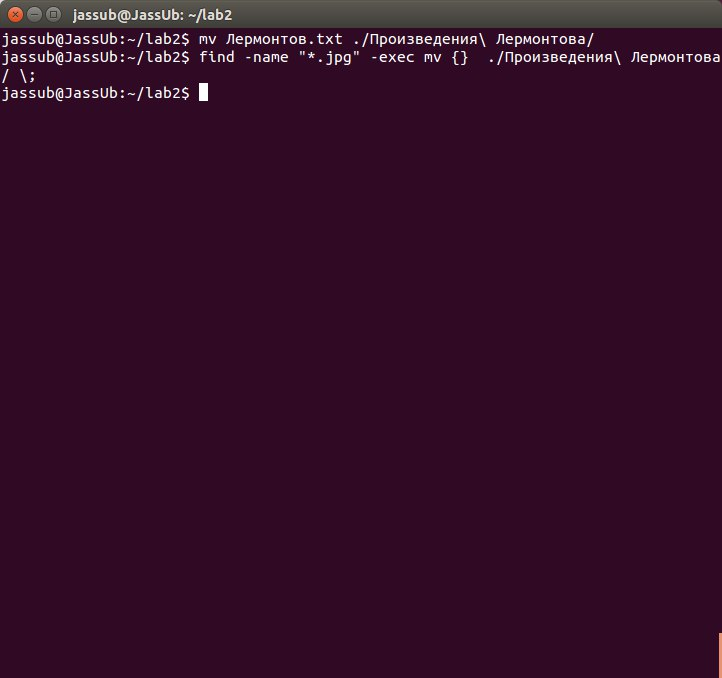
\includegraphics[scale=0.5]{3_4}
		\caption{Переносим .txt файл} 
		\label{pic:pic_1} % название для ссылок внутри кода
	\end{center}
\end{figure}

\begin{figure}[H]
	\begin{center}
		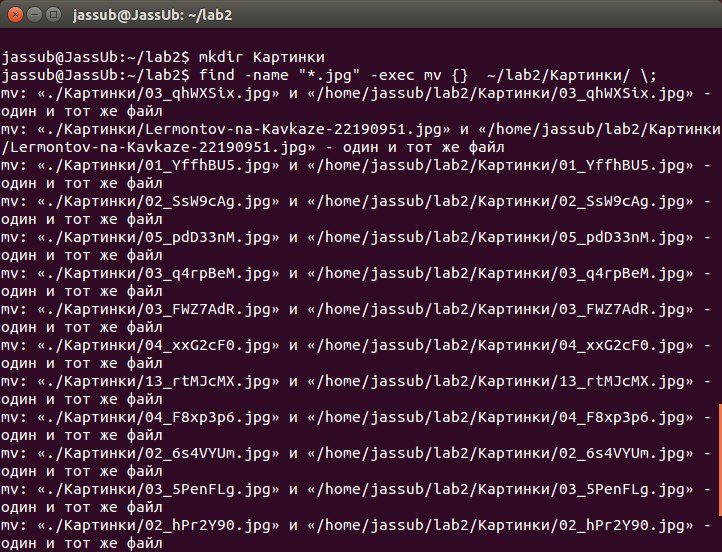
\includegraphics[scale=0.5]{3_5}
		\caption{Создаем директория Картинки с помощью команды mkdir. После производим поиск по нужному формату и переносим их в папку картинки.} 
		\label{pic:pic_1} % название для ссылок внутри кода
	\end{center}
\end{figure} 

\subsection{grep - утилита командной строки, которая находит на вводе строки, отвечающие заданному регулярному выражению, и выводит их, если вывод не отменён специальным ключом.}
\subsubsection{Параметр -с отключает стандартный способ вывода результата и вместо этого отображает только число обозначающее количество найденых строк}
\subsubsection{Параметр -i делает поиск регистронезависимым}

\begin{figure}[H]
	\begin{center}
		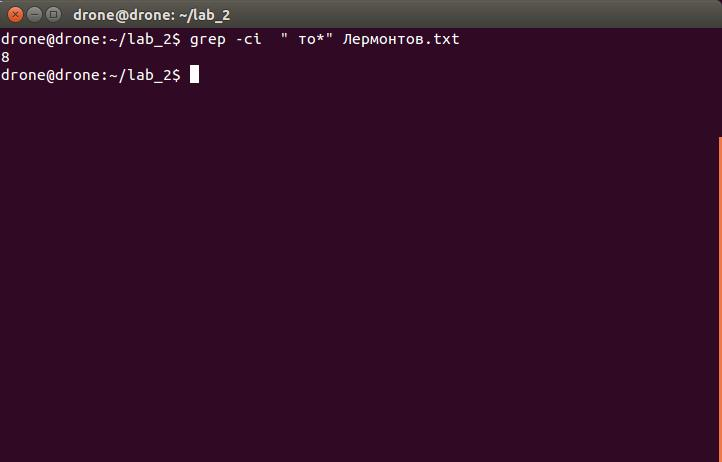
\includegraphics[scale=0.5]{3_}
		\caption{Подсчёт количества слов вида "то*"} 
		\label{pic:pic_1} % название для ссылок внутри кода
	\end{center}
\end{figure}

\section{Задание 4. Работа с архивами:}

\subsection{zip - утилита сжатия}

\subsubsection{Параметр -r добавляет все файлы в архив и указываем название архива и нужную папку}

\begin{figure}[H]
	\begin{center}
		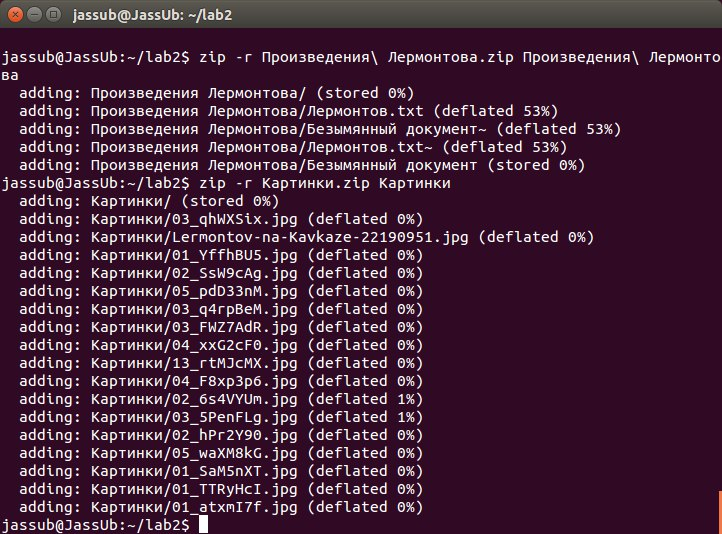
\includegraphics[scale=0.5]{4_1}
		\caption{Архивируем, используя zip} 
		\label{pic:pic_1} % название для ссылок внутри кода
	\end{center}
\end{figure}

\subsection{tar - наиболее распространенный архиватор, используемый в Linux-системах}

\subsubsection{Параметр -с служит для создания архива}
\subsubsection{Параметр -v необходим для расширенного вывода информации о выполненных действиях}
\subsubsection{Параметр -f выводит информацию извлекаемую из файла}

\begin{figure}[H]
	\begin{center}
		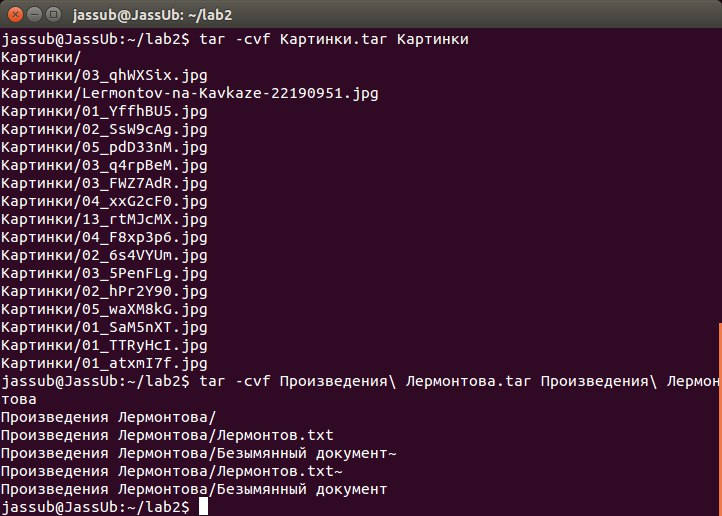
\includegraphics[scale=0.5]{4_2}
		\caption{Архивируем картинки, используя tar} 
		\label{pic:pic_1} % название для ссылок внутри кода
	\end{center}
\end{figure}

\subsection{tgz - архивирует нужную нам папку через два архиватора tar и gzip}

\begin{figure}[H]
	\begin{center}
		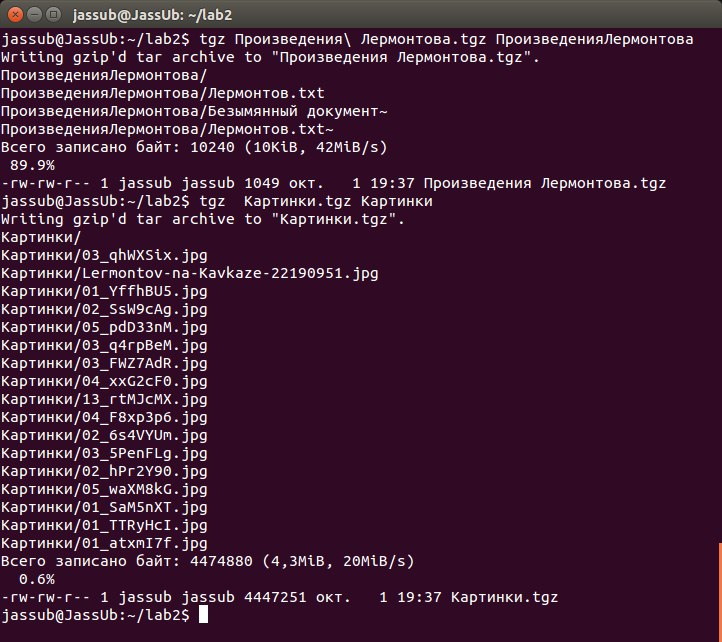
\includegraphics[scale=0.5]{4_4}
		\caption{Архивируем картинки, используя tar} 
		\label{pic:pic_1} % название для ссылок внутри кода
	\end{center}
\end{figure}

\subsection{Просмотр содержания архивов}

\begin{figure}[H]
	\begin{center}
		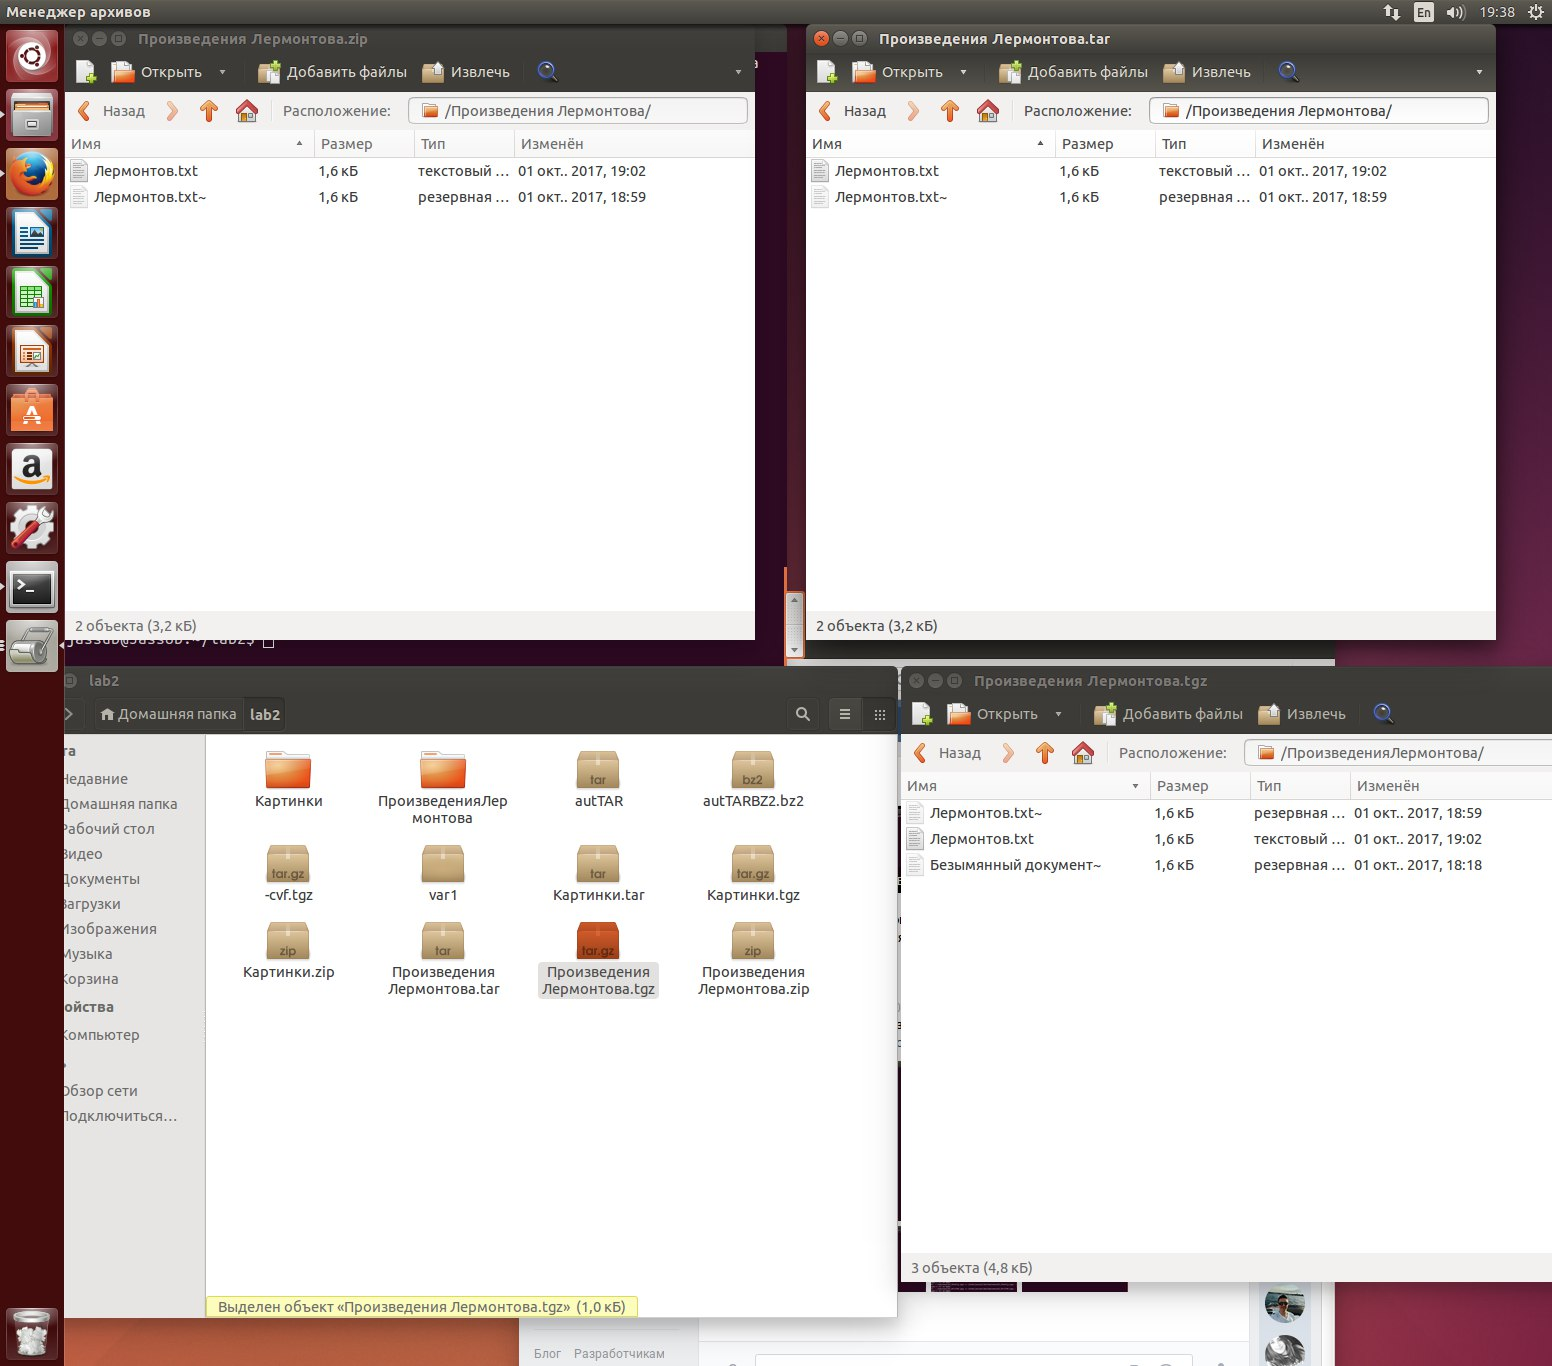
\includegraphics[scale=0.3]{4_5}
		\caption{Заархивированный .txt файл} 
		\label{pic:pic_1} % название для ссылок внутри кода
	\end{center}
\end{figure}

\begin{figure}[H]
	\begin{center}
		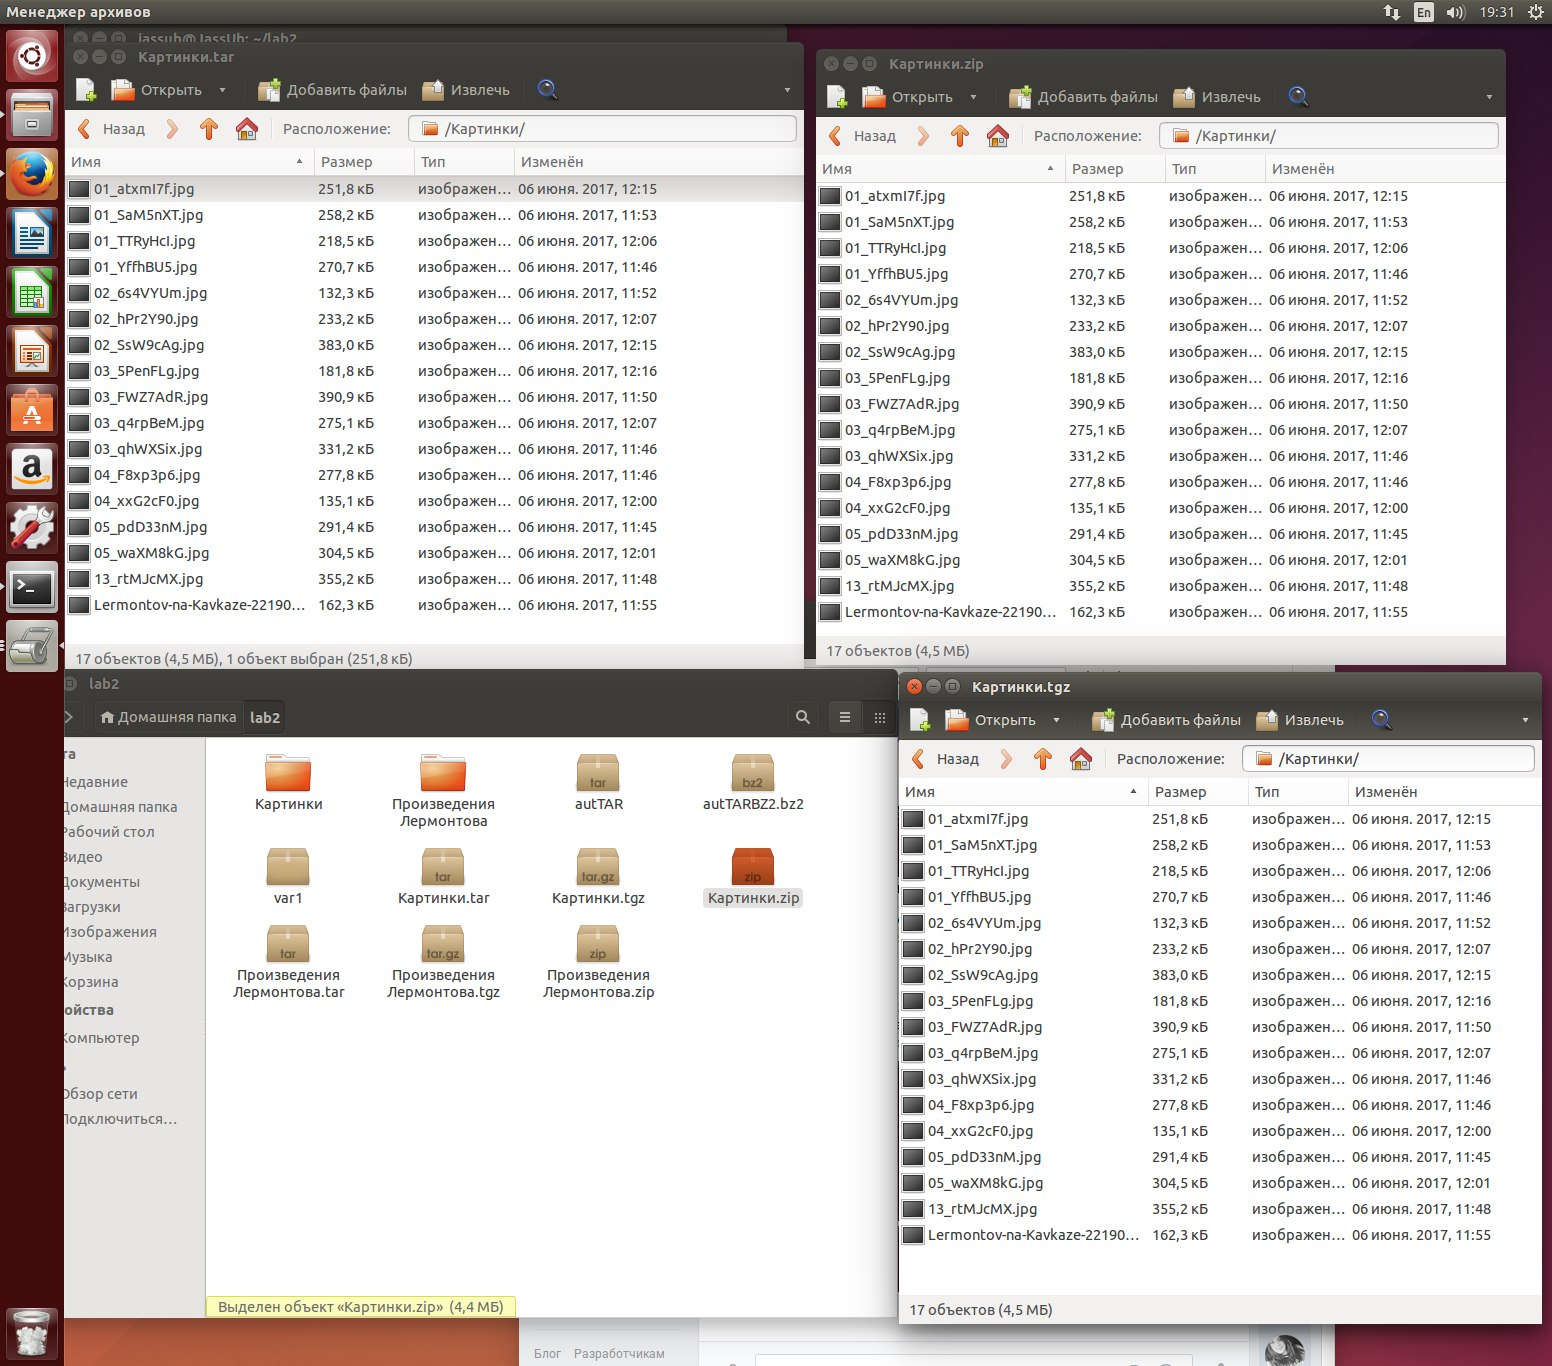
\includegraphics[scale=0.3]{4_6}
		\caption{Заархивированные картинки} 
		\label{pic:pic_1} % название для ссылок внутри кода
	\end{center}
\end{figure}

\section{Задание 5. Просмотр содержимого файлов:}

\begin{figure}[H]
	\begin{center}
		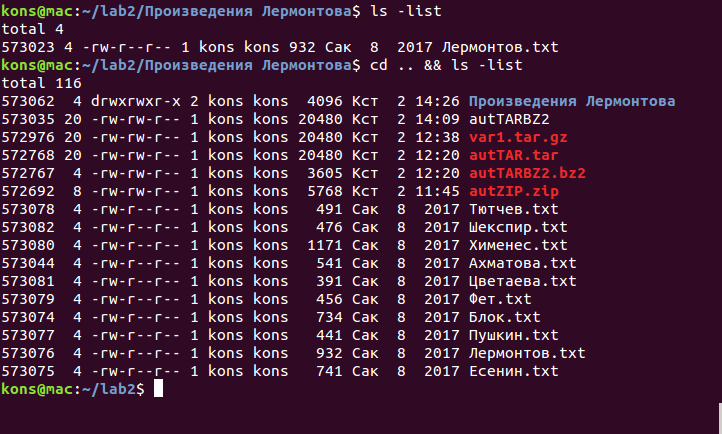
\includegraphics[scale=0.5]{5_1}
		\caption{Расширения файла в папке "Произведения Лермонтова" и файла извлеченного из .zip архива .txt} 
		\label{pic:pic_1} % название для ссылок внутри кода
	\end{center}
\end{figure}

\subsection{cat - утилита последовательно читает файлы и пишет их в стандартный вывод}

\subsubsection{Параметр -v выводит строки которые не удовлетворяют ключу}
\subsubsection{Параметр -n нумерует строки}

\begin{figure}[H]
	\begin{center}
		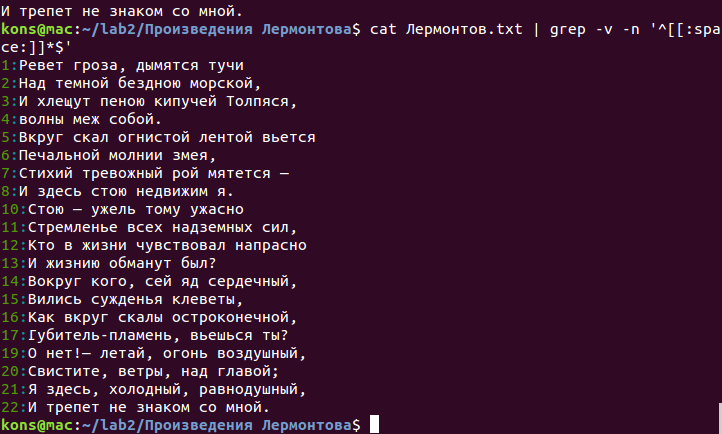
\includegraphics[scale=0.5]{5_2}
		\caption{С помощью утилиты cat выводим содержимое файла без пустых строк, нумеруем строки} 
		\label{pic:pic_1} % название для ссылок внутри кода
	\end{center}
\end{figure}

\subsection{more - утилита позволяет просмотреть содержимое файла. С помощью параметра -n можно вывести определенное количество строк на экран}

\begin{figure}[H]
	\begin{center}
		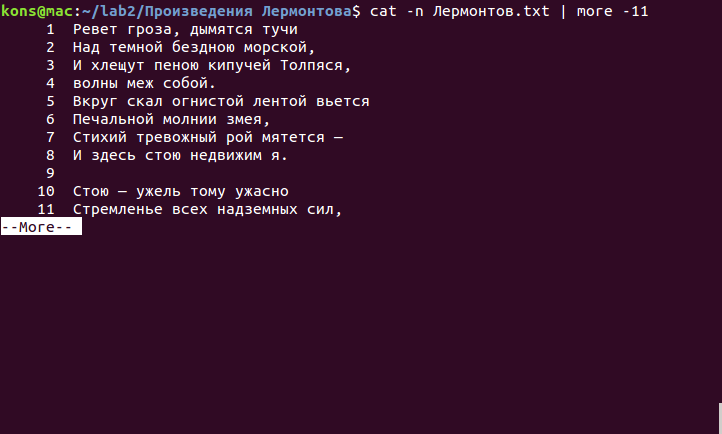
\includegraphics[scale=0.5]{5_6}
		\caption{Вывод текста} 
		\label{pic:pic_1} % название для ссылок внутри кода
	\end{center}
\end{figure}

\subsection{Утилита less, как и утилита more, используется для просмотра содержимого файлов}

\begin{figure}[H]
	\begin{center}
		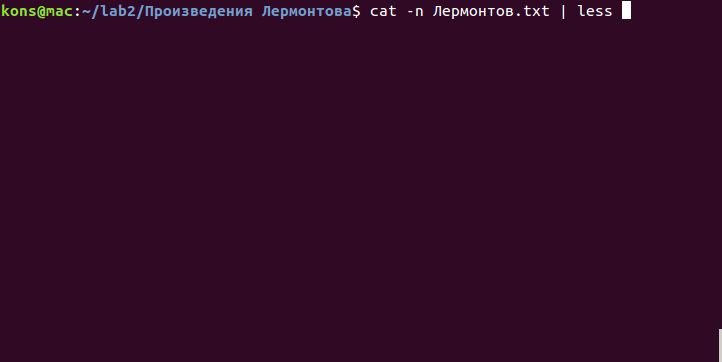
\includegraphics[scale=0.5]{5_4}
		\caption{Команда} 
		\label{pic:pic_1} % название для ссылок внутри кода
	\end{center}
\end{figure}
\begin{figure}[H]
	\begin{center}
		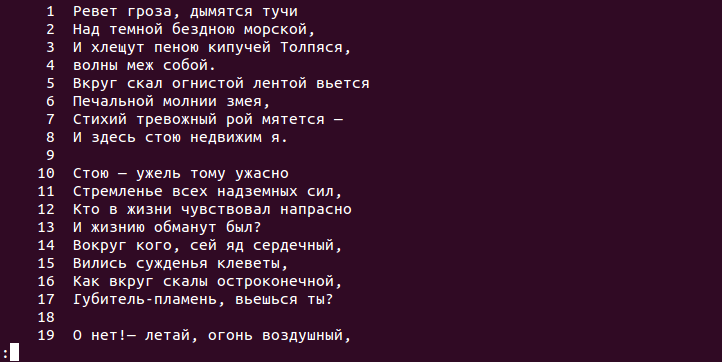
\includegraphics[scale=0.5]{5_5}
		\caption{Вывод текста} 
		\label{pic:pic_1} % название для ссылок внутри кода
	\end{center}
\end{figure}

\section{Задание 6. Управление правами доступа к файлам и каталогам:}

Размер файла в папке "Произведения Лермонтова" больше по сравнению с файлом в папке "lab2". Оба файла имеют одинаковые права. Владелец имеет права на чтение и запись, группа и все остальные имеют права только на чтение

\begin{figure}[H]
	\begin{center}
		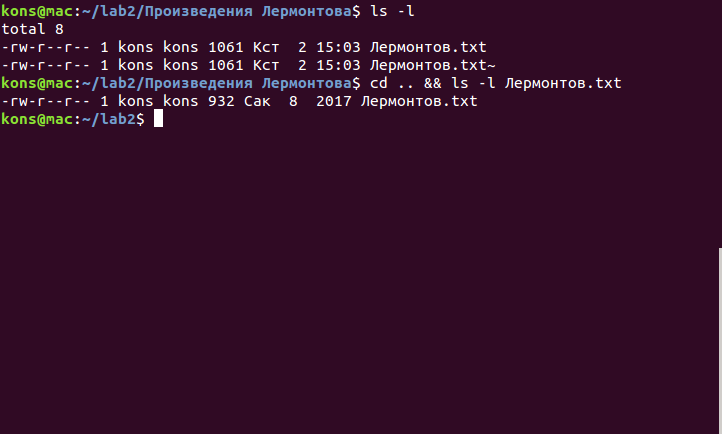
\includegraphics[scale=0.5]{6_1}
		\caption{} 
		\label{pic:pic_1} % название для ссылок внутри кода
	\end{center}
\end{figure}

\subsection{Удаляем права на чтение с помощью утилиты chmod, которая позволяет менять права доступа к директориям и файлам}

\subsubsection{Параметры go-r означают, что для группы и остальных, удаляются права на чтение. С помощью утилиты less имеется возможность просмотреть содержимое файла, так как эти действия производятся владельцем файла}

\begin{figure}[H]
	\begin{center}
		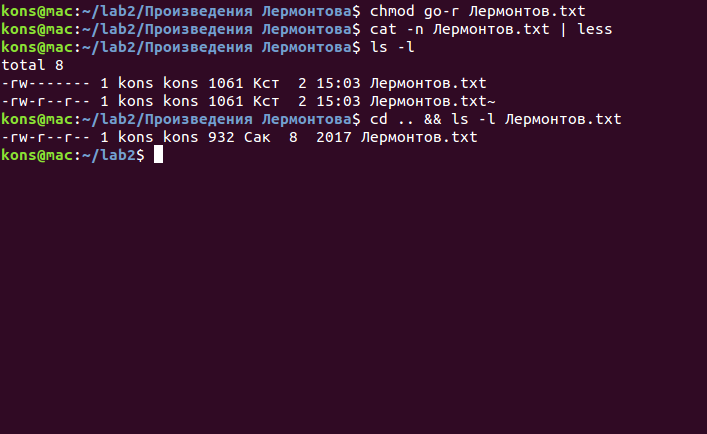
\includegraphics[scale=0.5]{6_2}
		\caption{} 
		\label{pic:pic_1} % название для ссылок внутри кода
	\end{center}
\end{figure}

\subsubsection{Параметры u-w означают, что для владельца файла удаляется право на запись}

\begin{figure}[H]
	\begin{center}
		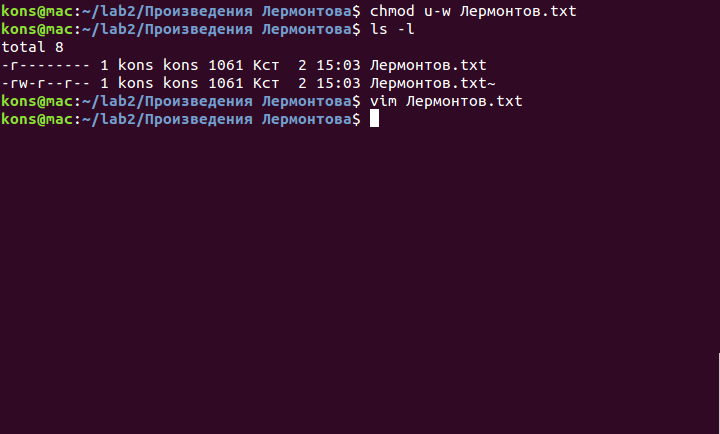
\includegraphics[scale=0.5]{6_3_1}
		\caption{} 
		\label{pic:pic_1} % название для ссылок внутри кода
	\end{center}
\end{figure}

\subsection{Добаляем права на запуск для группы и остальных пользователей. Запуск файла невозможен, так как у владельца файла отсутствуют права на запуск}

\begin{figure}[H]
	\begin{center}
		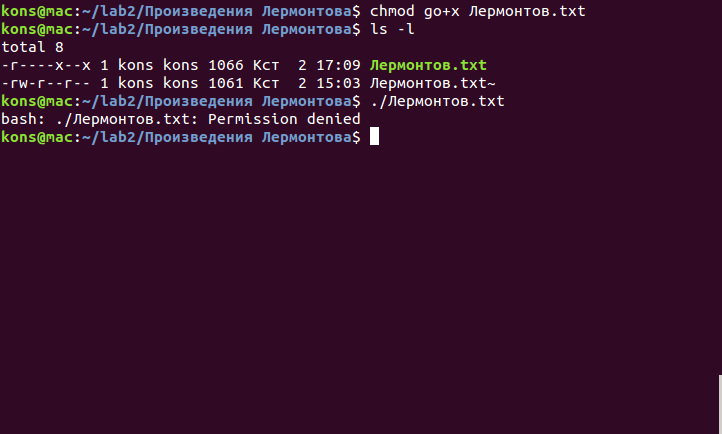
\includegraphics[scale=0.5]{6_4}
		\caption{} 
		\label{pic:pic_1} % название для ссылок внутри кода
	\end{center}
\end{figure}

\subsection{С помощью утилиты echo добавляем строчку в файл, проверяем права доступа. Владелец и группа пользователей имеют права на чтение и запись, остальные имеют права только на чтение. Добавляем права на запуск для владельца и группы в восьмиричной системе. Запуск удачен}

\begin{figure}[H]
	\begin{center}
		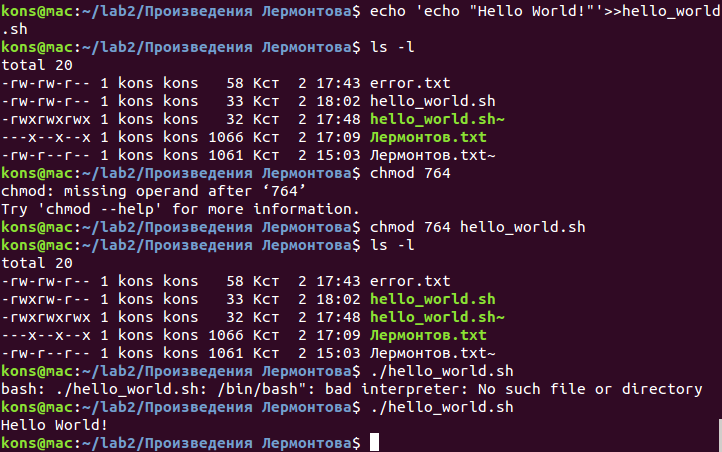
\includegraphics[scale=0.5]{6_5}
		\caption{} 
		\label{pic:pic_1} % название для ссылок внутри кода
	\end{center}
\end{figure}

\section{Задание 6. Команды для ввода/вывода данных. Перенаправление ввода/вывода:}

\subsection{С помощью команды chmod добавляем права на выполнение}

\begin{figure}[H]
	\begin{center}
		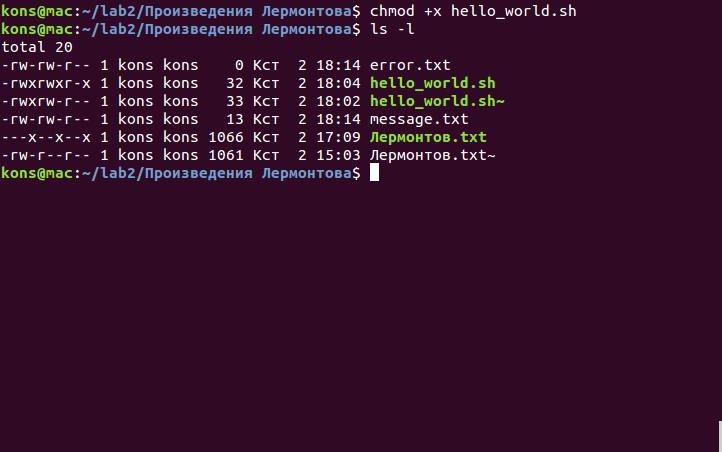
\includegraphics[scale=0.5]{7_1}
		\caption{} 
		\label{pic:pic_1} % название для ссылок внутри кода
	\end{center}
\end{figure}

\subsection{Перенаправляем вывод в файл message.txt и ошибки в файл error.txt. Файл с сообщениями содрежит строчку 'Hello World!', а файл с ошибками пуст}

\begin{figure}[H]
	\begin{center}
		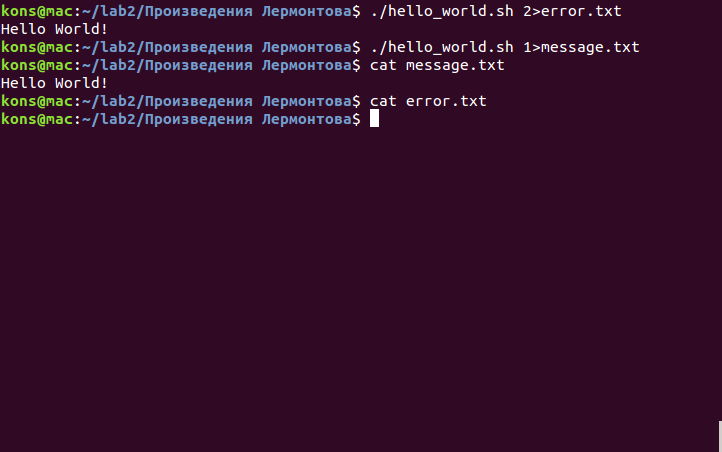
\includegraphics[scale=0.5]{7_2}
		\caption{} 
		\label{pic:pic_1} % название для ссылок внутри кода
	\end{center}
\end{figure}

\subsection{Используем входной поток с командой cat. Получаем строчку 'Hello World!' в терминале}

\begin{figure}[H]
	\begin{center}
		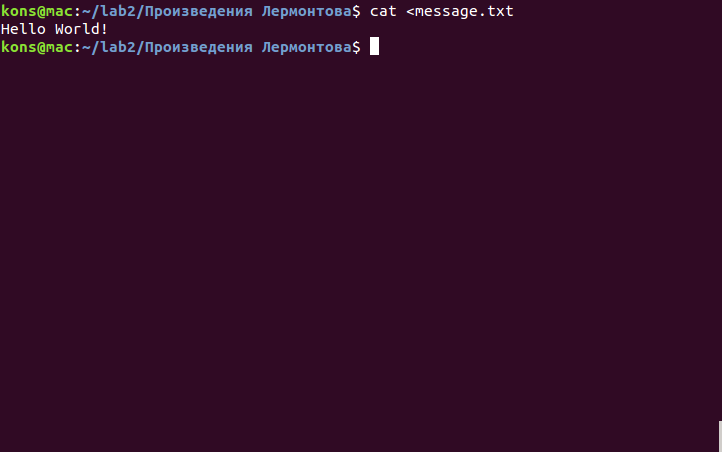
\includegraphics[scale=0.5]{7_3}
		\caption{} 
		\label{pic:pic_1} % название для ссылок внутри кода
	\end{center}
\end{figure}

\section{Вывод}
В данной лабораторной работе были изучены команды для скачивания файлов из Интернета, для работы с архивами, а также для поиска файлов и слов в файлах. 
\end{document}
